% ============================================================
%  BOUNDING AND APPROXIMATION
%  A chapter on the triangle inequality, distance management,
%  and the analyst's toolkit for controlling motion.
% ============================================================

% ---- Breadcrumb ----
\begin{tcolorbox}[
  colback=gray!6,
  colframe=gray!40,
  arc=2pt,
  left=8pt, right=8pt, top=6pt, bottom=6pt,
  title={\small\textbf{Where You Are in the Journey}},
  fonttitle=\small\bfseries
]
\begin{center}
\small
Number Systems
$\;\to\;$ Sequences and Convergence
$\;\to\;$ \textbf{Bounding and Approximation}
$\;\to\;$ Continuity
$\;\to\;$ Integration
\end{center}

\medskip
\noindent\textbf{How we got here.}
The previous chapters built the real numbers and introduced sequences.
You can now write down what it means for $x_n \to L$: for every
$\varepsilon > 0$, eventually $|x_n - L| < \varepsilon$.
The definition is clear. What is not yet clear is how to \emph{prove}
it in any situation more complicated than a constant sequence.

\medskip
\noindent\textbf{What this chapter builds.}
This chapter is a field manual for controlling distances.
The central tool is the triangle inequality — which most students
have seen but few have learned to use deliberately.
We develop a systematic vocabulary: target distances, known small
quantities, pivots, constant bounds. With this vocabulary in hand,
most $\varepsilon$-proofs become routine applications of a small
number of identifiable patterns.

\medskip
\noindent\textbf{Where this leads.}
Every technique here reappears — unchanged in structure — in the proofs of
continuity, differentiability, uniform convergence, and completeness.
Learning the patterns once, deeply, pays dividends throughout the rest
of the course.
\end{tcolorbox}
\vspace{1em}

% ---- Roadmap ----
\subsection*{Structural Roadmap}

\begin{center}
  \textbf{Conceptual Framework
  $\;\longrightarrow\;$ Analyst's Checklist
  $\;\longrightarrow\;$ Triangle Inequality Toolkit
  $\;\longrightarrow\;$ Worked Templates}
\end{center}

The global progression is:
\begin{enumerate}
  \item \textbf{Analysis as control of motion} — what kind of object
        is an $\varepsilon$-proof really controlling?
  \item \textbf{Three types of distance} — a classification that tells
        you which proof pattern to reach for.
  \item \textbf{The analyst's diagnostic checklist} — four questions
        that model a bounding problem before any algebra begins.
  \item \textbf{The triangle inequality toolkit} — seven named
        decompositions with geometric interpretations.
  \item \textbf{Preliminary bounding} — why the quotient and reciprocal
        cases require a separate safety-margin step.
  \item \textbf{The $\varepsilon/n$ splitting convention} — the
        mechanical rule for dividing an error budget between independent terms.
  \item \textbf{Scratch work vs.\ finished proof} — how analysts actually
        find their $\delta$ or $N$ before writing the clean argument.
  \item \textbf{Worked proof templates} — fully annotated models for sums,
        products, reciprocals, and continuity.
\end{enumerate}

\begin{remark*}[Primary sources]
Abbott \S1.2, \S2.3; Tao Analysis~I \S6.1, \S9.3--9.4;
Pugh \S1 (triangle inequality), \S2 (metric spaces);
Lebl \S1.3, \S2.1.
\end{remark*}

\clearpage

% ============================================================
%  PART I — CONCEPTUAL FRAMEWORK
% ============================================================

\section{Analysis as Control of Motion}
\label{sec:analysis-as-control}

\subsection{The Central Idea}

There is a useful way to think about what analysis is doing.

\begin{tcolorbox}[colback=thmbox, colframe=thmborder, arc=2pt,
  left=8pt, right=8pt, top=6pt, bottom=6pt]
\textbf{Guiding Principle.}
Analysis studies how quantities \emph{move}, and proofs
\emph{control that motion} using bounds.
In a metric space $(X,d)$, motion is measured by distance:
\[
  d(x,z) \;\le\; d(x,y) + d(y,z).
\]
The triangle inequality says that the direct distance between two points
cannot exceed the distance obtained by travelling through intermediate points.
This principle allows complicated motion to be decomposed into simpler pieces.
\end{tcolorbox}

\medskip

Bounding arguments therefore answer one question:
\begin{center}
  \emph{How far apart can these objects get from one another?}
\end{center}

\subsection{Moving vs.\ Static Objects}

The first step in any bounding problem is to classify every expression
in sight as either \emph{moving} or \emph{static}.

\medskip
\noindent\textbf{Static objects} do not change during the argument.
They are fixed reference points: constants, limits, function values
at a specific point.
\[
  L,\quad M,\quad f(a),\quad 0,\quad \tfrac{|L|}{2}.
\]
Geometrically, static objects are nails in the plane — they do not move.

\medskip
\noindent\textbf{Moving objects} vary with an index or parameter.
\[
  x_n,\quad y_n,\quad f(x),\quad g(t).
\]
Geometrically, moving objects are points tracing a path through the space.

\medskip
\noindent\textbf{Example.} When we write $x_n \to L$, the sequence $x_n$
is moving and the limit $L$ is a fixed nail.
The expression $|x_n - L|$ measures the distance between the moving
point and its target.
The proof's job is to show this distance can be made as small as we like.

\begin{remark*}[Why this matters]
Beginners often write down the definition of convergence correctly but
then stare at the page without knowing what to do next.
The reason is usually that they have not yet identified which objects
are moving and which are fixed.
Once that classification is made, the structure of the proof often
becomes clear immediately.
\end{remark*}

\subsection{Three Types of Distance}
\label{sec:three-distance-types}

Almost every expression in analysis can be interpreted as one of three
types of distance. Recognising the type tells you which tool to reach for.

\medskip

\noindent\textbf{Type 1 — Moving point vs.\ static target.}
\[
  |x_n - L|, \qquad |f(x) - f(a)|, \qquad |s_n - s|.
\]
One object moves; the other is a fixed reference.
This is the fundamental notion of convergence and continuity.
Bounding strategy: control how close the moving point gets to the nail.

\medskip

\noindent\textbf{Type 2 — Moving point vs.\ moving point.}
\[
  |x_n - y_n|, \qquad |x_m - x_n|.
\]
Both objects move. Their distance may fluctuate unpredictably —
we cannot control either one directly.
Bounding strategy: \emph{compare both objects to a shared static
reference point}.
\[
  |x_n - y_n|
  = |(x_n - L) + (L - y_n)|
  \le |x_n - L| + |y_n - L|.
\]
The distance between two moving points is controlled by their
individual distances to a common anchor.
(This is the Cauchy and squeeze-type strategy.)

\medskip

\noindent\textbf{Type 3 — Distance between distances.}
\[
  \bigl|d(x,z) - d(y,z)\bigr|.
\]
This measures how much the distance to $z$ changes as we move from
$x$ to $y$.
The reverse triangle inequality gives:
\[
  \bigl|d(x,z) - d(y,z)\bigr| \le d(x,y).
\]
Interpretation: distances cannot change faster than the points move.

\medskip

\noindent\textbf{Each type connects to a recognisable theorem.}

\smallskip
\begin{center}
\renewcommand{\arraystretch}{1.4}
\begin{tabular}{l l l}
\toprule
\textbf{Type} & \textbf{Example theorem} & \textbf{Key move} \\
\midrule
Type 1: moving vs.\ static  & Definition of $x_n \to L$
  & bound $|x_n - L|$ directly \\
Type 2: moving vs.\ moving  & Cauchy criterion
  & introduce shared anchor $L$ \\
Type 3: distance of distances & $|\,\cdot\,|$ is continuous
  & RTI bounds the fluctuation \\
\bottomrule
\end{tabular}
\end{center}

\medskip

\begin{remark*}[Error propagation]
Each type records how errors \emph{propagate} through an expression.
Type~1 says: the error in $x_n$ directly controls the error in the
output.
Type~2 says: two independent errors add when we compare two moving
quantities.
Type~3 says: the error in a distance is bounded by the error in the
underlying points.
Bounding arguments are, at root, a precise accounting of how input
errors combine to produce output errors.
\end{remark*}

\begin{figure}[h]
\centering
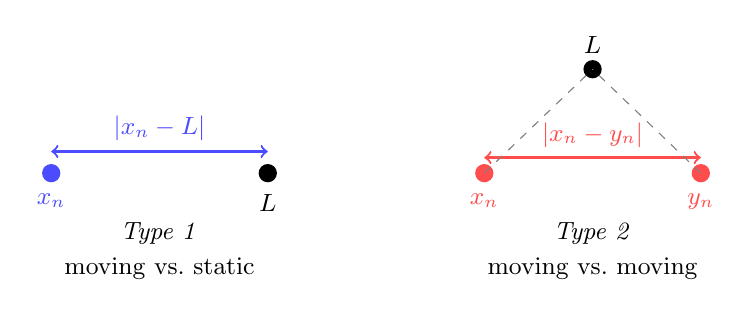
\begin{tikzpicture}[scale=1.1]
  % Type 1
  \begin{scope}[xshift=0cm]
    \fill[blue!70] (0,0) circle (3pt) node[below=4pt]{\small $x_n$};
    \fill[black]   (2.5,0) circle (3pt) node[below=4pt]{\small $L$};
    \draw[<->,thick,blue!70] (0,0.25) -- (2.5,0.25)
      node[midway,above]{\small $|x_n-L|$};
    \node at (1.25,-0.7){\small \textit{Type 1}};
    \node at (1.25,-1.1){\small moving vs.\ static};
  \end{scope}
  % Type 2
  \begin{scope}[xshift=5cm]
    \fill[red!70]  (0,0)   circle (3pt) node[below=4pt]{\small $x_n$};
    \fill[red!70]  (2.5,0) circle (3pt) node[below=4pt]{\small $y_n$};
    \fill[black]   (1.25,1.2) circle (3pt) node[above=2pt]{\small $L$};
    \draw[<->,thick,red!70] (0,0.18) -- (2.5,0.18)
      node[midway,above]{\small $|x_n-y_n|$};
    \draw[dashed,gray] (0,0) -- (1.25,1.2);
    \draw[dashed,gray] (2.5,0) -- (1.25,1.2);
    \node at (1.25,-0.7){\small \textit{Type 2}};
    \node at (1.25,-1.1){\small moving vs.\ moving};
  \end{scope}
\end{tikzpicture}
\caption{Types 1 and 2. In Type 2, the shared anchor $L$ is introduced
to separate the two uncontrolled motions into two individually
controllable pieces.}
\end{figure}

\subsection{Why the Triangle Inequality Dominates Analysis}
\label{sec:why-ti-dominates}

Everything in this chapter flows from a single inequality.
It is worth pausing to understand why that one inequality is so powerful,
and what would break without it.

\medskip

\noindent\textbf{The triangle inequality is a structural axiom, not just
a computational fact.}

When we say $x_n \to L$, we mean that the distance $d(x_n, L)$ can be
made arbitrarily small.
When we then ask whether $x_n + y_n \to L + M$, we are asking whether
the operation of addition is \emph{compatible} with the notion of limit.
The answer is yes — and the only reason it is yes is the triangle
inequality.

The proof of the sum rule is, at its core, one line:
\[
  d(x_n + y_n,\; L + M)
  \;\le\;
  d(x_n, L) + d(y_n, M).
\]
Each term on the right goes to zero by hypothesis.
Therefore so does the left.

Remove the triangle inequality and this argument collapses entirely.
In a ``space'' where distances do not satisfy the triangle inequality,
two sequences could each converge individually while their sum diverges.
The concept of limit would no longer be stable under the most basic
algebraic operations, and analysis as a subject would be unworkable.

\medskip

\noindent\textbf{What the triangle inequality is really saying.}

The inequality $d(A, C) \le d(A, B) + d(B, C)$ says:
\emph{local errors combine predictably}.
If $A$ is close to $B$, and $B$ is close to $C$, then $A$ is close to $C$.
This transitivity of closeness is so natural that it feels obvious —
but it is a non-trivial constraint on what ``distance'' means,
and not every function that looks like a distance satisfies it.

The triangle inequality is precisely the axiom that enforces this
transitivity. Every proof in this chapter is an application of that
single idea: decompose a hard distance into two easy distances,
each of which is controlled by a hypothesis.

\medskip

\noindent\textbf{Where this structure reappears.}

The techniques in this chapter are not special to the real line.
They work in any setting where distance satisfies the triangle
inequality — which is exactly the definition of a metric space.

\begin{tcolorbox}[colback=gray!6, colframe=gray!40, arc=2pt,
  left=8pt, right=8pt, top=6pt, bottom=6pt,
  title={\small\textbf{The Triangle Inequality Across Mathematics}},
  fonttitle=\small\bfseries]
\small
\renewcommand{\arraystretch}{1.45}
\begin{tabular}{l l l}
\toprule
\textbf{Setting} & \textbf{Triangle inequality} & \textbf{What it enables} \\
\midrule
$\mathbb{R}$ with $|\cdot|$
  & $|x - z| \le |x - y| + |y - z|$
  & all of real analysis \\
Metric space $(X, d)$
  & $d(x,z) \le d(x,y) + d(y,z)$
  & limits, continuity, completeness \\
Normed space $(V, \|\cdot\|)$
  & $\|u + v\| \le \|u\| + \|v\|$
  & functional analysis, Banach spaces \\
Lipschitz functions
  & $|f(x)-f(y)| \le K|x-y|$
  & controlled composition of limits \\
\bottomrule
\end{tabular}
\end{tcolorbox}

\medskip

Each row of this table is the triangle inequality in disguise.
A normed space is a vector space where lengths satisfy the triangle
inequality; a Banach space is a complete normed space.
A Lipschitz function is one that cannot stretch distances by more
than a fixed factor $K$ — which means the triangle inequality
propagates through composition without blowup.

\begin{remark*}[What to take away now]
You do not need to understand metric spaces or Banach spaces yet.
The point is simply this: every manipulation you learn in this chapter
is valid in all of those settings without modification.
When you later meet uniform convergence, or sequences of functions,
or contraction mappings, the proofs will look identical in structure
to the ones here — because they are all applications of the same
underlying axiom.
Recognising the triangle inequality in a new setting is the moment
a proof stops being mysterious.
\end{remark*}

\clearpage

% ============================================================
%  PART II — THE ANALYST'S CHECKLIST
% ============================================================

\section{The Analyst's Diagnostic Checklist}
\label{sec:analyst-checklist}

Experienced analysts do not start writing inequalities immediately when
they encounter a bounding problem. They first run through a short mental
checklist that \emph{models the geometry of the problem} before any algebra
begins. Beginners fail precisely because they skip this step.

\begin{tcolorbox}[colback=gray!6, colframe=gray!40, arc=2pt,
  left=8pt, right=8pt, top=6pt, bottom=6pt,
  title={\small\textbf{The Four Questions}},
  fonttitle=\small\bfseries]
\begin{enumerate}
  \item \textbf{What is the target distance?}
        Read it from the definition being proved. Do not guess.
  \item \textbf{What distances are already known to be small?}
        These are the given hypotheses expressed as closeness conditions.
  \item \textbf{What intermediate point will expose those distances?}
        This is the \emph{pivot}. Choosing it is the creative step.
  \item \textbf{What quantities can be replaced by constants?}
        Convergent sequences are bounded; use that bound.
\end{enumerate}
\end{tcolorbox}

\medskip

These questions separate two distinct tasks:
\begin{itemize}
  \item \textbf{Modelling the geometry} of the problem (Questions 1--3).
  \item \textbf{Executing algebraic manipulations} (Question 4 onwards).
\end{itemize}
The modelling step is where most of the real work happens.
Once the right picture is in place, the algebra is routine.

\subsection{Question 1 — Identifying the Target Distance}

The target distance always comes directly from the \emph{definition}
of the property being proved. There is no creativity here — just reading.

\begin{center}
\renewcommand{\arraystretch}{1.4}
\begin{tabular}{ll}
\toprule
\textbf{Property being proved} & \textbf{Target distance} \\
\midrule
$x_n \to L$                      & $|x_n - L|$ \\
$x_n + y_n \to L + M$            & $|(x_n+y_n)-(L+M)|$ \\
$x_n y_n \to LM$                 & $|x_n y_n - LM|$ \\
$f$ continuous at $a$            & $|f(x) - f(a)|$ \\
$(x_n)$ is Cauchy                & $|x_m - x_n|$ \\
\bottomrule
\end{tabular}
\end{center}

\begin{remark*}[Why not multiply the individual errors?]
A natural first instinct is to bound $|x_n y_n - LM|$ by
$|x_n - L| \cdot |y_n - M|$.
This is wrong: $|x_n - L|\cdot|y_n - M|$ measures
\emph{area spanned by two errors}, not the distance between $x_n y_n$
and $LM$.
There is no algebraic identity connecting these two quantities directly.
The target distance must be the one stated in the definition — nothing else.
\end{remark*}

\subsection{Question 2 — Known Small Distances}

Once the target is clear, list every distance you already know can be
made small. These come from the hypotheses.

\medskip
\begin{center}
\renewcommand{\arraystretch}{1.4}
\begin{tabular}{ll}
\toprule
\textbf{Hypothesis} & \textbf{Known small quantity} \\
\midrule
$x_n \to L$ & $|x_n - L| \to 0$ \\
$y_n \to M$ & $|y_n - M| \to 0$ \\
$|x - a| < \delta$ & $|x - a|$ can be made small by choice of $\delta$ \\
$(x_n)$ Cauchy   & $|x_m - x_n|$ for $m,n \ge N$ \\
\bottomrule
\end{tabular}
\end{center}

\medskip

The proof's job is to \emph{rewrite the target distance in terms of
these known small quantities}.

\subsection{Question 3 — The Pivot}

When the target expression does not already contain the known small
quantities, we \emph{add and subtract} a carefully chosen intermediate
value — the \textbf{pivot}.

\begin{tcolorbox}[colback=propbox, colframe=propborder, arc=2pt,
  left=8pt, right=8pt, top=6pt, bottom=6pt,
  title={\small\textbf{Definition (Pivot)}},
  fonttitle=\small\bfseries]
A \textbf{pivot} is an intermediate value $B$ inserted into the
expression $|A - C|$ by writing
\[
  |A - C| = |A - B + B - C| \le |A - B| + |B - C|.
\]
The pivot is chosen so that the two resulting pieces contain the
known small distances identified in Question~2.
\end{tcolorbox}

\medskip

\begin{tcolorbox}[colback=gray!6, colframe=gray!40, arc=2pt,
  left=8pt, right=8pt, top=6pt, bottom=6pt,
  title={\small\textbf{The Algebraic Skeleton}},
  fonttitle=\small\bfseries]
The manipulation underlying every pivot is the identity
\[
  A - C \;=\; (A - B) + (B - C).
\]
This is simply ``add and subtract the same quantity $B$''.
The triangle inequality then converts the identity into an inequality.
Inserting a pivot is not a trick — it is the systematic application
of this one algebraic move, with $B$ chosen to expose the known-small
quantities.
\end{tcolorbox}

\medskip

\noindent\textbf{Pivot selection heuristic.}
Choose the pivot so that each resulting term contains
\emph{exactly one known-small quantity}.
This is the invariant that all good pivots satisfy:
after applying the triangle inequality, every piece of the bound
isolates a single small factor, leaving everything else to be
replaced by a fixed constant.

\medskip

\noindent\textbf{The standard pivot for a product.}

Target: $|x_n y_n - LM|$.
Known small: $|x_n - L|$ and $|y_n - M|$.

The pivot $x_n M$ works because it allows us to split:
\[
  x_n y_n - LM
  = \underbrace{x_n y_n - x_n M}_{\text{contains }y_n - M}
  + \underbrace{x_n M - LM}_{\text{contains }x_n - L}.
\]
Each piece now contains exactly one of the known small quantities.

\medskip

\noindent\textbf{The pivot is symmetric — two valid choices.}

The product pivot is not unique.
The alternative pivot $y_n L$ gives an equally valid decomposition:
\[
  x_n y_n - LM
  = \underbrace{x_n y_n - y_n L}_{\text{contains }x_n - L}
  + \underbrace{y_n L - LM}_{\text{contains }y_n - M}
  = y_n(x_n - L) + L(y_n - M).
\]
The resulting bound is:
\[
  |x_n y_n - LM| \;\le\; |y_n|\,|x_n - L| + |L|\,|y_n - M|.
\]
Both terms are still linear in the known-small quantities.
The only difference is which sequence gets bounded by a constant:
with pivot $x_n M$ you bound $|x_n|$; with pivot $y_n L$ you bound
$|y_n|$.

\begin{center}
\renewcommand{\arraystretch}{1.4}
\begin{tabular}{l l l}
\toprule
\textbf{Pivot} & \textbf{Decomposition} & \textbf{Bounded factor} \\
\midrule
$x_n M$ & $x_n(y_n - M) + M(x_n - L)$ & $|x_n| \le B$ \\
$y_n L$ & $y_n(x_n - L) + L(y_n - M)$ & $|y_n| \le B'$ \\
\bottomrule
\end{tabular}
\end{center}

\begin{remark*}[Why standard texts use $x_n M$]
Both pivots are structurally correct.
The minor asymmetry is bookkeeping: $L$ and $M$ are already constants
and need no bounding, but $x_n$ and $y_n$ are moving and each requires
invoking boundedness of a convergent sequence.
If one of $|L|$ or $|M|$ is zero, the $+1$ trick is needed in the
denominator during scratch work to avoid division by zero.
The pivot that places the \emph{non-zero} limit as the constant
multiplier on one term can slightly simplify the scratch — but this
is a bookkeeping preference, not a structural difference.
Either pivot leads to a valid proof by the same mechanism.
\end{remark*}

\begin{remark*}[Rectangle geometry of the two pivots]
The rectangle diagram makes the symmetry visible.
The L-shaped region between the target rectangle $LM$ and the current
rectangle $x_n y_n$ has \emph{two} natural corners at which to split:
pivot $x_n M$ is the corner where you hold the width $x_n$ fixed and
first adjust the height from $y_n$ to $M$, then adjust the width;
pivot $y_n L$ is the corner where you hold the height $y_n$ fixed and
first adjust the width from $x_n$ to $L$, then adjust the height.
Both corners produce an overlapping two-strip cover of the L-shaped
region with the same qualitative structure — only the labelling of
which strip is ``horizontal'' and which is ``vertical'' swaps.
\end{remark*}

\medskip

\noindent\textbf{Why linearity in the small quantities is the goal.}

After a pivot decomposition, the ideal outcome is a bound of the form
\[
  |A - C| \;\le\; C_1 \cdot |x_n - L| \;+\; C_2 \cdot |y_n - M|,
\]
where $C_1$ and $C_2$ are fixed constants.
Understanding \emph{why} this form is desirable is more important than
any individual manipulation.

The reason is this: we have direct, explicit control over $|x_n - L|$
and $|y_n - M|$.
By the definition of convergence, for any target size $r > 0$ we can
choose $N$ large enough that both are smaller than $r$ for all $n \ge N$.
A fixed constant $C_1$ does not interfere with this — we simply require
$|x_n - L| < \varepsilon / (2C_1)$ instead of $|x_n - L| < \varepsilon/2$,
which is equally achievable.

The structure $C \cdot (\text{small})$ therefore means:
\begin{itemize}
  \item the constant $C$ is no obstacle — we absorb it into the
        $\varepsilon$ budget by dividing,
  \item the small quantity goes to zero by hypothesis,
  \item so the entire term goes to zero.
\end{itemize}
This is the complete logical chain that makes the proof work.
Every other manipulation in this chapter is in service of arriving
at exactly this form.

\medskip

\noindent\textbf{Why quadratic terms break this logic.}

Suppose instead the bound contains a term like
$(x_n - L)(y_n - M)$ — a \emph{product} of two small quantities.
This seems even smaller, so why is it a problem?

The issue is not whether the term goes to zero (it does),
but whether the proof has a clean, workable structure.
With a quadratic term, the size of the bound is controlled by
$\varepsilon^2$ rather than $\varepsilon$.
To make $(x_n - L)(y_n - M) < \varepsilon$ it suffices to make
each factor less than $\sqrt{\varepsilon}$ — but the $\varepsilon/n$
bookkeeping now involves square roots, the argument becomes
case-sensitive (what if one factor is very large and the other very
small?), and the method does not extend cleanly to three or more terms.

More fundamentally: every additional power of $\varepsilon$ means
one more piece of bookkeeping, one more case to check, one more
place to make an error.
Linearity is not just convenient — it is the form that makes
$\varepsilon$-arguments \emph{mechanical}.
A bound that is linear in the small quantities can always be closed
by the same routine split-and-absorb procedure.
A bound that involves products of small quantities requires
new reasoning each time.

\medskip

\noindent\textbf{Why wrong pivots fail — a case study.}

Suppose we try the pivot $LM$ instead (i.e.\ do not insert anything
and just bound $|x_n y_n - LM|$ directly).
We obtain nothing useful because neither $|x_n y_n|$ nor $|LM|$
separately contains the known small quantities.

Alternatively, suppose we try to split as
$x_n y_n - LM = (x_n - L)(y_n - M) + L(y_n - M) + M(x_n - L)$.
This is algebraically valid — but the first term
$(x_n - L)(y_n - M)$ is quadratic in the small quantities.
As explained above, this breaks the linearity that makes the
$\varepsilon/n$ procedure routine.
The standard pivot $x_n M$ avoids this entirely: it produces only
terms that are linear in $|x_n - L|$ and $|y_n - M|$.

\medskip

The lesson, stated precisely:
\begin{tcolorbox}[colback=gray!6, colframe=gray!40, arc=2pt,
  left=8pt, right=8pt, top=6pt, bottom=6pt]
A good pivot produces a bound of the form
$\sum_i C_i \cdot (\text{known-small}_i)$
where each $C_i$ is a fixed constant and each known-small quantity
appears \emph{to the first power only}.
This form is the target of all the manipulations in this chapter,
because it is the exact form that the $\varepsilon/n$ splitting
procedure is designed to close.
\end{tcolorbox}

\subsection{Question 4 — Replacing Terms by Constants}

After inserting a pivot, one piece will typically contain a moving term
(such as $x_n$) multiplying a small quantity.
We cannot leave $x_n$ there — it is not a fixed bound.
But we know convergent sequences are bounded:

\begin{tcolorbox}[colback=thmbox, colframe=thmborder, arc=2pt,
  left=8pt, right=8pt, top=6pt, bottom=6pt,
  title={\small\textbf{Boundedness of Convergent Sequences}},
  fonttitle=\small\bfseries]
If $x_n \to L$, then there exists $B > 0$ such that $|x_n| \le B$
for all $n$.
In particular, we may take $B = |L| + 1$ (once $n$ is large enough
for $|x_n - L| < 1$).
\end{tcolorbox}

\medskip

This converts $|x_n| \cdot |y_n - M|$ into $B \cdot |y_n - M|$,
which is \emph{constant times small} — exactly what we need.

\begin{remark*}[The analyst's pattern]
After applying Question~4, every term in the bound has the form
\[
  C \cdot (\text{known small quantity}),
\]
where $C$ is a fixed constant.
Each such term can be made less than $\varepsilon/k$ for appropriate
choice of $N$ or $\delta$, and the terms are then summed using
the $\varepsilon/n$ convention (see \S\ref{sec:eps-splitting}).
\end{remark*}

\clearpage

% ============================================================
%  PART III — THE TRIANGLE INEQUALITY TOOLKIT
% ============================================================

\section{The Triangle Inequality Toolkit}
\label{sec:ti-toolkit}

\begin{tcolorbox}[colback=gray!6, colframe=gray!40, arc=2pt,
  left=8pt, right=8pt, top=6pt, bottom=6pt,
  title={\small\textbf{Triangle Inequality Toolkit — Quick Reference}},
  fonttitle=\small\bfseries]
\small
\begin{tabular}{l l l}
\toprule
\textbf{Name} & \textbf{Key identity / bound} & \textbf{When to use} \\
\midrule
TI-1 Sum        & $|(x - L) + (y - M)| \le |x - L| + |y - M|$ & limit of sums \\
TI-2 Difference & $|(x - L) - (y - M)| \le |x - L| + |y - M|$ & limit of differences \\
TI-3 Product    & $|xy - LM| \le |x|\,|y - M| + |M|\,|x - L|$ & limit of products \\
TI-4 Quotient   & $\displaystyle\left|\tfrac{1}{x} - \tfrac{1}{L}\right|
                    = \tfrac{|x - L|}{|x|\,|L|}$      & reciprocal limits \\
TI-5 Square     & $|x^2 - L^2| = |x - L|\,|x + L|$  & polynomial limits \\
TI-6 Poly diff  & $|x^2 - y^2| = |x - y|\,|x + y|$  & comparing two moving terms \\
TI-7 Iterated   & $|a_1 + \cdots + a_n| \le |a_1| + \cdots + |a_n|$ & sums of $n$ terms \\
\midrule
Lipschitz       & $|f(x) - f(y)| \le C\,|x - y|$    & continuity, contractions, norms \\
\midrule
RTI Reverse     & $\bigl||x| - |y|\bigr| \le |x - y|$ & safety margins, norm continuity \\
\bottomrule
\end{tabular}
\end{tcolorbox}

\medskip

\noindent\textbf{Scope of this toolkit.}
These seven rules form the core vocabulary for first-pass bounding
arguments in undergraduate real analysis.
Later you will meet other moves — supremum estimates, order squeezing,
monotonicity bounds, mean value theorem estimates, comparison arguments
— but almost all of them are built on top of what is here.

\medskip

\noindent\textbf{The Lipschitz pattern.}
Many proofs in analysis reduce to showing that a function satisfies
\[
  |f(x) - f(y)| \le C\,|x - y|
\]
for some fixed constant $C$.
Such functions are called \emph{Lipschitz}, and they automatically
preserve limits: if $x_n \to y$ then $f(x_n) \to f(y)$.
The absolute value function, all linear functions, and all contractions
are Lipschitz.
This pattern is the same constant-times-small structure that appears
throughout this chapter — recognising it unifies limit proofs,
continuity proofs, and fixed-point arguments under a single template.
The Lipschitz row in the table above is a reminder that the toolkit
extends beyond sequences.

\medskip

\noindent\textbf{Core principle.}
Every technique in this toolkit is simply a choice of pivot $B$ so that
the known small quantities appear after applying:
\[
  |A - C| \le |A - B| + |B - C|.
\]

\begin{figure}[h]
\centering
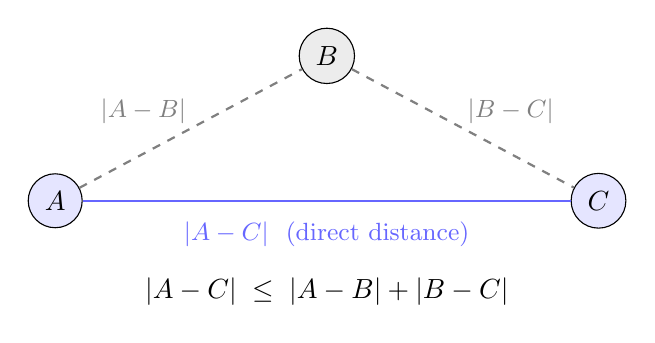
\begin{tikzpicture}[scale=1.15]
  % nodes
  \node (A) at (0,0)   [circle,draw,fill=blue!10,minimum size=18pt] {$A$};
  \node (B) at (3,1.6) [circle,draw,fill=gray!15,minimum size=18pt] {$B$};
  \node (C) at (6,0)   [circle,draw,fill=blue!10,minimum size=18pt] {$C$};
  % direct
  \draw[thick,blue!60] (A) -- (C)
    node[midway,below=4pt]{\small $|A-C|$ \ (direct distance)};
  % path
  \draw[thick,dashed,gray] (A) -- (B)
    node[midway,above left=-2pt]{\small $|A-B|$};
  \draw[thick,dashed,gray] (B) -- (C)
    node[midway,above right=-2pt]{\small $|B-C|$};
  % inequality label
  \node at (3,-1.0) {$|A-C|\;\le\;|A-B|+|B-C|$};
\end{tikzpicture}
\caption{The triangle inequality as a path: the direct distance is
never larger than any two-step detour through a pivot $B$.
Choosing the right $B$ is the entire art of bounding.}
\end{figure}

\subsection{TI-1 and TI-2 — Sum and Difference Decomposition}

\textbf{Setting.} Two sequences converge: $x_n \to L$ and $y_n \to M$.
We want to control $|(x_n + y_n) - (L+M)|$.

\textbf{Identity.}
\[
  (x_n + y_n) - (L+M) = (x_n - L) + (y_n - M).
\]

\textbf{Bound.}
\[
  |(x_n - L) + (y_n - M)| \le |x_n - L| + |y_n - M|.
\]

The total error is the sum of two independent errors, one for each
sequence. This is the simplest application of the triangle inequality,
and it is also an over-bound: the two errors could partially cancel
(if $x_n - L$ and $y_n - M$ have opposite signs), making the actual
error smaller than the right-hand side. Since we are proving an
inequality, that is fine — a bound that is sometimes too generous
is still a valid bound.

\begin{figure}[h]
\centering
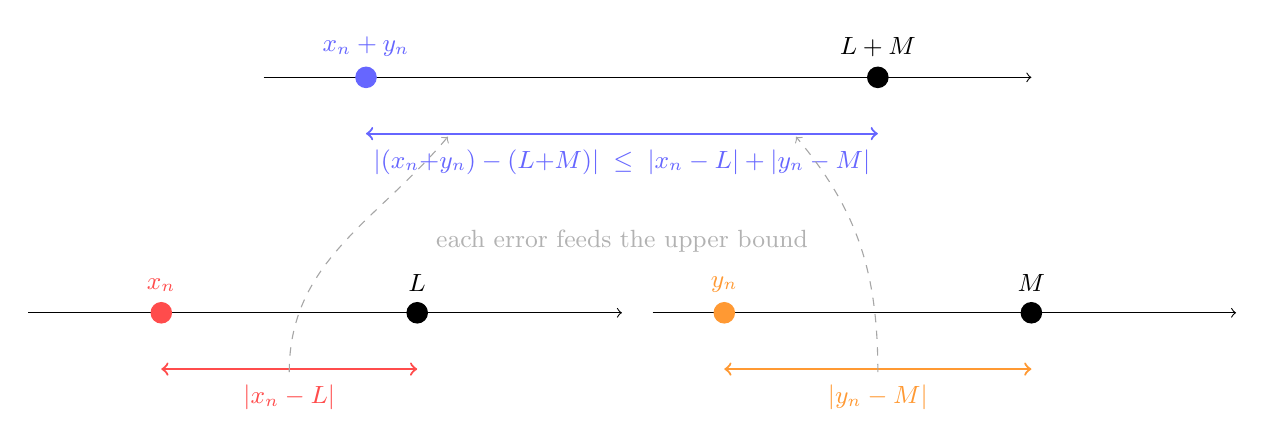
\begin{tikzpicture}[scale=1.3]

  % Two-row layout.
  % Row 1 (y=0): the two individual errors |x_n-L| and |y_n-M| on separate axes.
  % Row 2 (y=2.2): the combined sum error |(x_n+y_n)-(L+M)|.
  % Dashed arrows show the two pieces feeding the combined bound.

  % ---- Row 1a: x_n error ----
  \draw[->] (-0.3, 1.2) -- (5.5, 1.2);
  \fill[red!70]  (1.0, 1.2) circle (3pt) node[above=4pt] {\small $x_n$};
  \fill[black]   (3.5, 1.2) circle (3pt) node[above=4pt] {\small $L$};
  \draw[<->, thick, red!70] (1.0, 0.65) -- (3.5, 0.65)
    node[midway, below=2pt] {\small $|x_n - L|$};

  % ---- Row 1b: y_n error (shifted right to share axis) ----
  \draw[->] (5.8, 1.2) -- (11.5, 1.2);
  \fill[orange!80] (6.5, 1.2) circle (3pt) node[above=4pt] {\small $y_n$};
  \fill[black]     (9.5, 1.2) circle (3pt) node[above=4pt] {\small $M$};
  \draw[<->, thick, orange!80] (6.5, 0.65) -- (9.5, 0.65)
    node[midway, below=2pt] {\small $|y_n - M|$};

  % ---- Row 2: combined error ----
  \draw[->] (2.0, 3.5) -- (9.5, 3.5);
  \fill[blue!60] (3.0, 3.5) circle (3pt) node[above=4pt] {\small $x_n + y_n$};
  \fill[black]   (8.0, 3.5) circle (3pt) node[above=4pt] {\small $L + M$};
  \draw[<->, thick, blue!60] (3.0, 2.95) -- (8.0, 2.95)
    node[midway, below=2pt]
      {\small $|(x_n{+}y_n)-(L{+}M)| \;\le\; |x_n-L| + |y_n-M|$};

  % ---- Dashed arrows from the two pieces up to the combined bar ----
  \draw[->, dashed, gray!70] (2.25, 0.62) to[out=90, in=230] (3.8, 2.92);
  \draw[->, dashed, gray!70] (8.0,  0.62) to[out=90, in=310] (7.2, 2.92);

  % ---- "feeds bound" annotation ----
  \node[gray!60] at (5.5, 1.9) {\small each error feeds the upper bound};

\end{tikzpicture}
\caption{Sum error decomposition. The total error $|(x_n+y_n)-(L+M)|$
(blue) is bounded by the sum of the two independent errors
$|x_n - L|$ (red) and $|y_n - M|$ (orange).
The bound may over-count when the two errors have opposite sign and
partially cancel, but since we only need an inequality this is harmless.}
\end{figure}

The difference case TI-2 is identical in structure:
\[
  |(x_n - y_n) - (L-M)| = |(x_n - L) - (y_n - M)|
  \le |x_n - L| + |y_n - M|.
\]


\subsection{TI-3 — Product Decomposition}

\textbf{Setting.} $x_n \to L$, $y_n \to M$. Control $|x_n y_n - LM|$.

\textbf{The key identity} (with pivot $x_n M$):
\[
  x_n y_n - LM
  = x_n y_n - x_n M + x_n M - LM
  = x_n(y_n - M) + M(x_n - L).
\]

\textbf{Bound:}
\[
  |x_n y_n - LM|
  \le |x_n|\,|y_n - M| + |M|\,|x_n - L|.
\]

Because $x_n \to L$, the sequence $(x_n)$ is bounded: $|x_n| \le B$.
Hence:
\[
  |x_n y_n - LM| \le B|y_n - M| + |M|\,|x_n - L|.
\]
Each term is \emph{constant times small quantity}.

\begin{figure}[h]
\centering
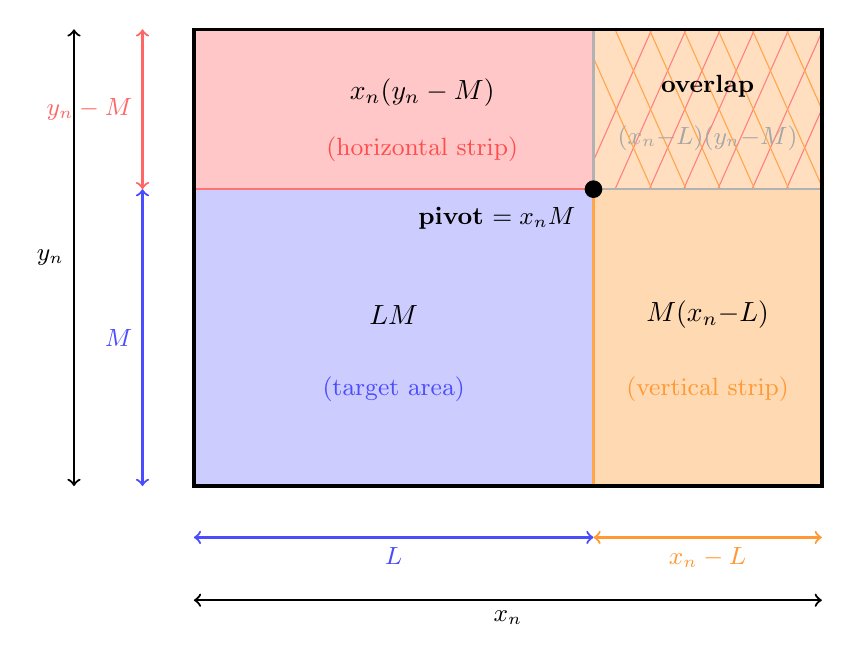
\begin{tikzpicture}[scale=1.45]

  % Coordinates:  L=3.5, x_n=5.5, M=2.6, y_n=4.0
  % The two strips OVERLAP on the corner square [3.5,5.5]x[2.6,4.0].
  % Draw order: blue target, then red full-width top band,
  % then orange full-height right strip, then double-shade the overlap corner.

  % ---- (1) target rectangle: L x M (blue) ----
  \fill[blue!20] (0,0) rectangle (3.5,2.6);
  \draw[blue!60, thick] (0,0) rectangle (3.5,2.6);
  \node at (1.75,1.5)   {$LM$};
  \node[blue!70] at (1.75,0.85) {\small (target area)};

  % ---- (2) horizontal strip: FULL width x_n, height (y_n-M) (red) ----
  % spans [0,5.5] x [2.6,4.0] — covers both left part AND corner
  \fill[red!22]  (0,2.6) rectangle (5.5,4.0);
  \draw[red!55, thick] (0,2.6) rectangle (5.5,4.0);
  \node at (2.0, 3.45) {$x_n(y_n - M)$};
  \node[red!70] at (2.0, 2.95) {\small (horizontal strip)};

  % ---- (3) vertical strip: width (x_n-L), FULL height M (orange) ----
  % spans [3.5,5.5] x [0,2.6] — covers both bottom part AND corner
  \fill[orange!30] (3.5,0) rectangle (5.5,2.6);
  \draw[orange!70, thick] (3.5,0) rectangle (5.5,2.6);
  \node at (4.5,1.5)   {$M(x_n{-}L)$};
  \node[orange!80] at (4.5,0.85) {\small (vertical strip)};

  % ---- (4) overlap corner: double-shade with hatching ----
  % Already red from step 2; add orange over it to show double-coverage
  \fill[orange!25] (3.5,2.6) rectangle (5.5,4.0);
  % Crosshatch pattern to signal overlap
  \begin{scope}
    \clip (3.5,2.6) rectangle (5.5,4.0);
    \foreach \x in {3.3,3.6,...,6.0} {
      \draw[red!50, thin] (\x,2.4) -- (\x+0.8,4.2);
    }
    \foreach \x in {3.3,3.6,...,6.0} {
      \draw[orange!70, thin] (\x,4.2) -- (\x+0.8,2.4);
    }
  \end{scope}
  \draw[gray!60, thick] (3.5,2.6) rectangle (5.5,4.0);
  \node[black] at (4.5,3.5)  {\small \textbf{overlap}};
  \node[gray!70] at (4.5,3.05) {\small $(x_n{-}L)(y_n{-}M)$};

  % ---- (5) outer border ----
  \draw[black, very thick] (0,0) rectangle (5.5,4.0);

  % ---- (6) pivot dot ----
  \fill[black] (3.5,2.6) circle (2.2pt);
  \node[below left=3pt] at (3.5,2.6)
    {\small \textbf{pivot} $= x_n M$};

  % ---- dimension arrows: widths ----
  \draw[<->, thick, blue!70]   (0,-0.45)  -- (3.5,-0.45)
    node[midway, below] {\small $L$};
  \draw[<->, thick, orange!80] (3.5,-0.45) -- (5.5,-0.45)
    node[midway, below] {\small $x_n - L$};
  \draw[<->, thick, black]     (0,-1.0)   -- (5.5,-1.0)
    node[midway, below] {\small $x_n$};

  % ---- dimension arrows: heights ----
  \draw[<->, thick, blue!70]  (-0.45,0)   -- (-0.45,2.6)
    node[midway, left] {\small $M$};
  \draw[<->, thick, red!60]   (-0.45,2.6) -- (-0.45,4.0)
    node[midway, left] {\small $y_n - M$};
  \draw[<->, thick, black]    (-1.05,0)   -- (-1.05,4.0)
    node[midway, left] {\small $y_n$};

\end{tikzpicture}
\caption{%
The rectangle picture for $|x_n y_n - LM|$ with overlapping strips.
The \textcolor{blue!70}{blue} rectangle is the target area $LM$.
The \textcolor{red!60}{red} band (full width $x_n$, height $y_n - M$)
and the \textcolor{orange!70}{orange} strip (width $x_n - L$, full height $M$)
together \emph{over-cover} the L-shaped difference region: their
\textbf{overlap} (the corner square, crosshatched) is counted twice.
Since we are proving an \emph{inequality}, this double-counting is
harmless — the bound $x_n|y_n-M| + |M||x_n-L|$ is slightly too large,
but a generous upper bound is still a valid upper bound.}
\end{figure}

\begin{remark*}[Why the overlap is a feature, not a bug]
The standard two-term decomposition
\[
  x_n y_n - LM \;=\; x_n(y_n-M) + M(x_n-L)
\]
does \emph{not} tile the L-shaped region exactly.
The horizontal strip uses the full width $x_n$, not just $L$,
so it extends into the corner square $(x_n - L)(y_n-M)$ — and the
vertical strip also covers that same corner.
The corner is counted twice.

The alternative that \emph{does} tile exactly is the three-term version:
\[
  x_n y_n - LM \;=\; L(y_n-M) \;+\; M(x_n-L) \;+\; (x_n-L)(y_n-M).
\]
This is an equality — no overlap, no waste — but the price is the
quadratic term $(x_n-L)(y_n-M)$, which requires separate treatment
(an additional $\delta$-case or a product-of-smalls argument).

The standard decomposition \emph{deliberately} pays the price of
over-counting the corner in order to eliminate the quadratic term.
The slack in the inequality — the fact that we only need
$\le$ and not $=$ — is what makes this exchange legal.
Each strip then contains exactly one small quantity multiplied by one
bounded factor, which is precisely the linear form the
$\varepsilon/n$ procedure requires.
\end{remark*}

\begin{tcolorbox}[colback=gray!6, colframe=gray!40, arc=2pt,
  left=8pt, right=8pt, top=6pt, bottom=6pt,
  title={\small\textbf{The Reusable Triad (applies beyond products)}},
  fonttitle=\small\bfseries]
The product proof is an instance of a pattern that appears throughout
analysis whenever a moving term multiplies a small quantity:
\begin{enumerate}
  \item \textbf{Isolate one small term.}
        Rewrite the expression so that exactly one known-small
        quantity appears as a separate factor in each piece.
        (This is what the pivot achieves.)
  \item \textbf{Bound the rest by a constant.}
        Replace any remaining moving factor — a convergent sequence,
        a function value on a closed interval — with a fixed upper bound.
  \item \textbf{Spend the $\varepsilon$ budget.}
        Allocate $\varepsilon/(k \cdot C)$ to each small term
        (where $C$ is its constant multiplier), so the total is $\varepsilon$.
\end{enumerate}
\medskip
Once this triad is internalised, you can read off the proof strategy
for limits of products, compositions, Lipschitz functions, and many
others directly from the structure of the expression — before
writing a single inequality.
\end{tcolorbox}

\subsection{TI-4 — Quotient Decomposition and the Safety Margin}
\label{sec:safety-margin}

The quotient case is structurally different from TI-1 through TI-3.
It requires a \emph{preliminary bounding step} before any triangle
inequality can be applied.

\medskip

\noindent\textbf{Why division is dangerous.}
If $x_n \to 0$, then $1/x_n \to \infty$.
No matter how convergent $x_n$ is, the reciprocal blows up.
Before we can bound $|1/x_n - 1/L|$, we must ensure $x_n$ never
gets too close to $0$ — we need a \emph{safety margin}.

\medskip

\noindent\textbf{Establishing the safety margin.}
Suppose $x_n \to L$ with $L \ne 0$.
Apply the reverse triangle inequality (RTI):
\[
  |x_n|
  = |L - (L - x_n)|
  \ge |L| - |L - x_n|.
\]
Choose $N$ large enough that $|x_n - L| < |L|/2$ for all $n \ge N$.
Then:
\[
  |x_n| > |L| - \tfrac{|L|}{2} = \tfrac{|L|}{2} > 0.
\]

The denominator is now bounded away from zero, uniformly in $n \ge N$.
Taking reciprocals (which reverses inequalities for positive quantities):
\[
  \frac{1}{|x_n|} < \frac{2}{|L|}.
\]
This is the constant we need.

\medskip

\noindent\textbf{Now apply the triangle inequality.}
\[
  \left|\frac{1}{x_n} - \frac{1}{L}\right|
  = \frac{|L - x_n|}{|x_n||L|}
  = \frac{|x_n - L|}{|x_n| \cdot |L|}
  < \frac{2}{|L|} \cdot \frac{|x_n - L|}{|L|}
  = \frac{2}{|L|^2} \cdot |x_n - L|.
\]

\begin{figure}[h]
\centering
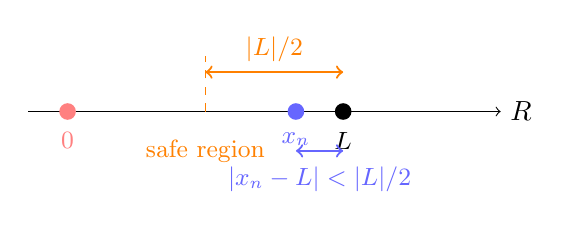
\begin{tikzpicture}[scale=1.0]
  \draw[->] (-0.5,0) -- (5.5,0) node[right]{$\mathbb{R}$};
  % zero
  \fill[red!50] (0,0) circle (3pt) node[below=4pt]{\small $0$};
  % L
  \fill[black]  (3.5,0) circle (3pt) node[below=4pt]{\small $L$};
  % safety margin
  \draw[<->,thick,orange] (3.5,0.5) -- (1.75,0.5)
    node[midway,above]{\small $|L|/2$};
  \draw[dashed,orange] (1.75,0) -- (1.75,0.7);
  \node[orange] at (1.75,-0.5){\small safe region};
  % x_n band
  \fill[blue!60] (2.9,0) circle (3pt) node[below=4pt]{\small $x_n$};
  \draw[<->,thick,blue!60] (3.5,-0.5) -- (2.9,-0.5)
    node[midway,below=2pt]{\small $|x_n-L|<|L|/2$};
\end{tikzpicture}
\caption{Safety margin technique. By keeping $x_n$ within distance
$|L|/2$ of $L$, we ensure $|x_n| > |L|/2$ and the reciprocal
$1/|x_n|$ stays bounded.}
\end{figure}

\begin{remark*}[Why TI-4 is structurally different]
Rules TI-1 through TI-3 and TI-5 through TI-7 all consist of:
(a)~choose a pivot, (b)~apply the triangle inequality.
TI-4 has an extra preliminary step: establish a lower bound on
$|x_n|$ before any triangle inequality is applied.
This step must happen first, or the subsequent manipulation is invalid.
When you see a reciprocal in a proof, always ask:
\emph{have I established the safety margin yet?}
\end{remark*}

\subsection{TI-5 and TI-6 — Factorization Decompositions}

\textbf{TI-5 (Square).}
\[
  x^2 - L^2 = (x - L)(x + L),
  \qquad
  |x^2 - L^2| = |x - L| \cdot |x + L|.
\]
Factorization isolates $|x - L|$ as a single factor.
The remaining factor $|x + L|$ is bounded on any bounded interval
containing the limit point — replace it by a constant.

\medskip

\textbf{TI-6 (Polynomial difference).}
\[
  x^2 - y^2 = (x-y)(x+y),
  \qquad
  |x^2 - y^2| = |x-y| \cdot |x+y|.
\]
Used when comparing two moving sequences, both converging.
Factorization converts nonlinear change into linear change.

\begin{remark*}[General polynomial case]
For a general polynomial $p(x) = a_0 + a_1 x + \cdots + a_k x^k$,
the identity
\[
  p(x) - p(L) = (x-L) \cdot q(x,L)
\]
holds for some polynomial $q$ (obtained by factoring out $(x-L)$).
On a bounded neighbourhood of $L$, $|q(x,L)|$ is bounded by a
constant, and the argument proceeds exactly as in TI-5.
\end{remark*}

\subsection{TI-7 — The Iterated Triangle Inequality}

When an expression involves the sum of $n$ terms, the triangle
inequality can be applied repeatedly:
\[
  |a_1 + a_2 + \cdots + a_n|
  \le |a_1| + |a_2| + \cdots + |a_n|.
\]

\textbf{Proof by induction.}
The base case $n = 2$ is the standard triangle inequality.
If the inequality holds for $n$ terms, then for $n+1$:
\[
  |a_1 + \cdots + a_n + a_{n+1}|
  \le |a_1 + \cdots + a_n| + |a_{n+1}|
  \le |a_1| + \cdots + |a_n| + |a_{n+1}|.
\]

\textbf{Geometric reading.}
Define partial sums $s_0 = 0$, $s_k = a_1 + \cdots + a_k$.
Then $|a_1 + \cdots + a_n| = |s_n - s_0|$ is the net displacement,
while $\sum |a_k| = \sum |s_k - s_{k-1}|$ is the total path length.
The inequality says: net displacement $\le$ total path length.

\begin{figure}[h]
\centering
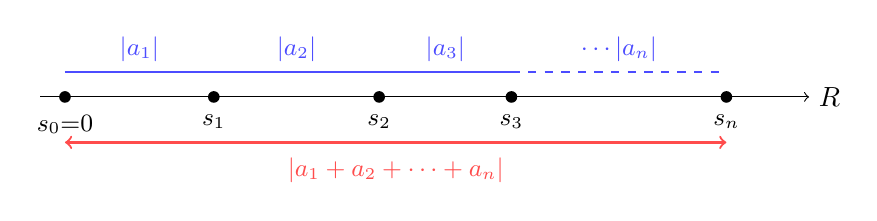
\begin{tikzpicture}[scale=1.05]
  \draw[->] (-0.3,0) -- (9.0,0) node[right]{$\mathbb{R}$};
  %
  \fill (0,0) circle (2pt) node[below=3pt]{\small $s_0{=}0$};
  \fill (1.8,0) circle (2pt) node[below=3pt]{\small $s_1$};
  \fill (3.8,0) circle (2pt) node[below=3pt]{\small $s_2$};
  \fill (5.4,0) circle (2pt) node[below=3pt]{\small $s_3$};
  \fill (8.0,0) circle (2pt) node[below=3pt]{\small $s_n$};
  %
  \draw[thick,blue!70] (0,0.3) -- (1.8,0.3)
    node[midway,above]{\small $|a_1|$};
  \draw[thick,blue!70] (1.8,0.3) -- (3.8,0.3)
    node[midway,above]{\small $|a_2|$};
  \draw[thick,blue!70] (3.8,0.3) -- (5.4,0.3)
    node[midway,above]{\small $|a_3|$};
  \draw[thick,blue!70,dashed] (5.4,0.3) -- (8.0,0.3)
    node[midway,above]{\small $\cdots|a_n|$};
  %
  \draw[<->,thick,red!70] (0,-0.55) -- (8.0,-0.55)
    node[midway,below=2pt]{\small $|a_1+a_2+\cdots+a_n|$};
\end{tikzpicture}
\caption{Iterated triangle inequality as a path diagram.
The total path length (blue, sum of step sizes) is at least
the net displacement (red, direct distance).}
\end{figure}

\subsection{RTI — The Reverse Triangle Inequality}

\begin{tcolorbox}[colback=propbox, colframe=propborder, arc=2pt,
  left=8pt, right=8pt, top=6pt, bottom=6pt,
  title={\small\textbf{Proposition (Reverse Triangle Inequality)}},
  fonttitle=\small\bfseries]
For all $x, y \in \mathbb{R}$:
\[
  \bigl|\,|x| - |y|\,\bigr| \le |x - y|.
\]
\end{tcolorbox}

\begin{remark*}[Fully quantified form]
$\forall x, y \in \mathbb{R},\quad \bigl|\,|x|-|y|\,\bigr| \le |x-y|$.
\end{remark*}

\begin{proof}
Apply the triangle inequality twice:
\[
  |x| = |(x - y) + y| \le |x-y| + |y|
  \quad\Rightarrow\quad
  |x| - |y| \le |x-y|.
\]
Swapping $x$ and $y$: $|y| - |x| \le |y - x| = |x - y|$.
Combining: $\bigl|\,|x|-|y|\,\bigr| \le |x-y|$.
\end{proof}

\begin{remark*}[When to use the RTI]
The reverse triangle inequality appears whenever you need a
\emph{lower} bound on a distance or magnitude.
The three most common situations are:
\begin{enumerate}
  \item Establishing the safety margin for reciprocals
        (ensuring $|x_n| \ge |L|/2$).
  \item Proving continuity of the norm or absolute value function
        ($|\,|f(x)| - |f(a)|\,| \le |f(x) - f(a)|$).
  \item Bounding differences of distances in metric spaces
        ($|d(x,z) - d(y,z)| \le d(x,y)$).
\end{enumerate}
\end{remark*}

\clearpage

% ============================================================
%  PART IV — SUPPORTING TECHNIQUES
% ============================================================

\section{The \texorpdfstring{$\varepsilon/n$}{Epsilon-over-n}
  Splitting Convention}
\label{sec:eps-splitting}

After applying the toolkit, a bound typically has the form:
\[
  |A - B| \le C_1 \cdot (\text{small}_1) + C_2 \cdot (\text{small}_2).
\]
We want the right-hand side to be less than $\varepsilon$.
The standard method is to make each term less than $\varepsilon/2$
separately.

\begin{tcolorbox}[colback=gray!6, colframe=gray!40, arc=2pt,
  left=8pt, right=8pt, top=6pt, bottom=6pt,
  title={\small\textbf{The \(\varepsilon/n\) Splitting Convention}},
  fonttitle=\small\bfseries]
If the bound contains $n$ independent error terms, allocate
$\varepsilon/n$ to each.
Specifically, if
\[
  |A - B| \le C_1\,|\text{small}_1| + C_2\,|\text{small}_2|,
\]
choose $N_1$ so that $|\text{small}_1| < \varepsilon/(2C_1)$ for $n \ge N_1$,
and $N_2$ so that $|\text{small}_2| < \varepsilon/(2C_2)$ for $n \ge N_2$.
Then for $n \ge \max(N_1, N_2)$:
\[
  |A - B|
  < C_1 \cdot \frac{\varepsilon}{2C_1} + C_2 \cdot \frac{\varepsilon}{2C_2}
  = \frac{\varepsilon}{2} + \frac{\varepsilon}{2}
  = \varepsilon.
\]
\end{tcolorbox}

\begin{remark*}[The constants cancel out]
Notice that $C_1$ and $C_2$ cancel exactly.
This means you do not need to find the sharpest possible constants —
any bound $C$ works, as long as it is fixed (independent of $n$).
The $\varepsilon/n$ convention automatically absorbs any finite
constant.
The specific value of the constant is irrelevant: it could be $B$,
or $|L| + 1$, or $47$.
Whatever positive constant appears out front, you put the same
constant in the denominator of your $\varepsilon$-fraction, and it
cancels to leave $\varepsilon/2$.
\end{remark*}

\begin{remark*}[$B$ and $|L|+1$ are interchangeable — and why the $+1$ appears]
When bounding $|x_n|$ in the product proof, two common choices are:
\begin{itemize}
  \item \textbf{Abstract bound $B$}: invoke the boundedness theorem to
        assert $|x_n| \le B$ for some unspecified $B > 0$.
        Then require $|y_n - M| < \varepsilon/(2B)$.
  \item \textbf{Explicit bound $|L|+1$}: use the fact that since
        $x_n \to L$, eventually $|x_n - L| < 1$, so
        $|x_n| \le |L| + 1$.
        Then require $|y_n - M| < \varepsilon/(2(|L|+1))$.
\end{itemize}
Both work by the same cancellation: $(|L|+1) \cdot \frac{\varepsilon}{2(|L|+1)} = \frac{\varepsilon}{2}$.
The explicit form $|L|+1$ is often preferred because it names the
constant in terms of something already in the problem rather than
introducing a fresh letter.

The $+1$ in $|L|+1$ also serves a second purpose: it guards against
$L = 0$.
If $L = 0$ then $|L| = 0$ and $\frac{\varepsilon}{2|L|}$ would be
undefined.
But $|L| + 1 \ge 1 > 0$ always, so division is safe regardless of
what $L$ is.

The same $+1$ guard appears in the other term: $\frac{\varepsilon}{2|M|+1}$
rather than $\frac{\varepsilon}{2|M|}$, for exactly the same reason —
$M$ might be zero.
When $M = 0$ the term $|M|\,|x_n - L|$ vanishes entirely, so no
actual work is needed for it; the $+1$ simply avoids a division-by-zero
in the formula without affecting the proof.

\medskip
\noindent The rule of thumb: \emph{any constant you intend to divide by
must be guaranteed positive.}
If it is a constructed bound like $B$ or $|L|+1$, positivity is
built in by construction.
If it is a given quantity like $|M|$ that could be zero, add $+1$.
\end{remark*}

\begin{remark*}[Unequal splitting]
The split need not be equal.
If one term is harder to control, allocate more budget to it:
for example, $\varepsilon/3$ and $2\varepsilon/3$, or any partition
summing to $\varepsilon$.
Equal splitting is the default because it is easiest to write.
\end{remark*}

\section{Scratch Work vs.\ Finished Proof}
\label{sec:scratch-work}

When a student reads a finished $\varepsilon$-proof, the choice of $N$
or $\delta$ appears as if by magic.
It does not appear by magic — it is found by \emph{working backwards}
in scratch.
But there is a further distinction, finer than scratch versus clean,
that is worth making explicit.

\medskip

\noindent\textbf{Two phases, not one.}

Every $\varepsilon$-proof is actually built in two separate phases,
which require different kinds of thinking:

\begin{enumerate}
  \item \textbf{The geometric phase.}
        Look at the expression.
        Identify its structure: what are the moving parts, what is the
        target, where does the known-small quantity live?
        Decide what the bound \emph{should} look like —
        which pivot to insert, which factors to replace by constants,
        what the linear form will be.
        This phase uses the diagnostic checklist (Questions 1--4)
        and geometric intuition.
        \emph{The triangle inequality is not needed here.}
        You are reading the geometry of the expression, not yet
        writing inequalities.

  \item \textbf{The analytic phase.}
        Now that you know what the bound looks like, formally justify it.
        Apply TI-1 through RTI to license each step.
        Invoke boundedness theorems.
        Run the $\varepsilon/n$ split to close the budget.
        This phase is largely mechanical once the geometric phase
        is complete.
        \emph{Its only job is to transcribe what you already know
        into rigorous inequality chains.}
\end{enumerate}

\medskip

The goal of scratch work is to \emph{complete the geometric phase}.
Once you know what the bound will look like — once you have identified
the pivot, the constants, and the linear structure — the analytic phase
is just transcription.
Most of the difficulty students experience with $\varepsilon$-proofs
comes from attempting the analytic phase without having completed the
geometric phase first: they start writing inequalities before they know
where they are going.

\medskip

\noindent\textbf{The workflow.}
\begin{enumerate}
  \item \textbf{Geometric scratch:} Run the diagnostic checklist.
        Identify target, known-small quantities, pivot, and constants.
        Write down what the bound will look like.
        No triangle inequality yet — just structure recognition.
  \item \textbf{Analytic scratch:} Work backwards from the bound
        to find $N$ or $\delta$.
        Ask: ``What would I need to be true for this bound to be
        less than $\varepsilon$?'' Solve for the threshold.
  \item \textbf{Clean proof:} Write the proof forwards.
        State $N$ or $\delta$ up front.
        Apply the toolkit steps in order.
        Conclude.
\end{enumerate}

\medskip

\noindent\textbf{Example: finding $N$ for the product limit.}

\textit{Scratch work.} We need:
\[
  B|y_n - M| + |M|\,|x_n - L| < \varepsilon.
\]
It suffices to make each term less than $\varepsilon/2$:
\[
  |y_n - M| < \frac{\varepsilon}{2B}, \qquad
  |x_n - L| < \frac{\varepsilon}{2|M|+1}.
  \quad\text{(The $+1$ avoids division by zero if $M=0$.)}
\]
By convergence of $y_n$, $\exists N_1$ such that $n \ge N_1
\Rightarrow |y_n - M| < \varepsilon/(2B)$.
By convergence of $x_n$, $\exists N_2$ such that $n \ge N_2
\Rightarrow |x_n - L| < \varepsilon/(2|M|+1)$.
Set $N = \max(N_1, N_2)$.

\textit{Now write the clean proof using this $N$.}

\begin{remark*}[Scratch work is never shown]
Scratch work is for the writer, not the reader.
The finished proof begins ``Let $\varepsilon > 0$.
Choose $N$ such that \ldots'' and proceeds forwards.
The backwards reasoning that found $N$ is tacitly present
but never written out in the final document.
\end{remark*}

\begin{remark*}[One constraint on scratch work]
Scratch work is allowed to be informal, but inequalities must
remain valid throughout.
A common error is to \emph{assume the conclusion} during scratch:
writing $|x_n y_n - LM| < \varepsilon$ at the top and then
manipulating it as if it were already known.
This produces a circular argument.
Scratch work runs \emph{backwards from what we need} — it does not
assume what we are trying to prove.
\end{remark*}

\clearpage

% ============================================================
%  PART V — COMMON FAILURE MODES
% ============================================================

\section{Common Failure Modes}
\label{sec:failure-modes}

The following mistakes are extremely common in early $\varepsilon$-proofs.
Each one has a specific cause and a specific fix.
Reading this section before attempting your first proofs is worth doing;
returning to it when a proof refuses to close is worth doing too.

\begin{tcolorbox}[colback=gray!6, colframe=gray!40, arc=2pt,
  left=8pt, right=8pt, top=6pt, bottom=6pt,
  title={\small\textbf{Pre-Proof Checklist}},
  fonttitle=\small\bfseries]
Before writing the final proof, confirm:
\begin{itemize}
  \item[$\square$] I have written down the correct target expression
                   (from the definition, not from intuition).
  \item[$\square$] My pivot introduces the known small quantities
                   into both resulting pieces.
  \item[$\square$] Every moving factor has been replaced by a constant.
  \item[$\square$] I have established a denominator safety margin
                   \emph{before} bounding any reciprocal.
  \item[$\square$] My $\varepsilon/n$ split was chosen \emph{after}
                   reading what the final inequality looks like.
\end{itemize}
\end{tcolorbox}

\medskip

\noindent\textbf{FM-1 \quad Choosing a pivot that introduces no known small quantities.}

\textit{What it looks like.}
You insert an intermediate term, apply the triangle inequality,
and obtain two pieces --- but neither piece contains $|x_n - L|$
or $|y_n - M|$.
The bound is valid but useless.

\textit{Example.}
Trying to bound $|x_n y_n - LM|$ by writing
\[
  |x_n y_n - LM| = |x_n y_n - x_n L + x_n L - LM|
  \le |x_n||y_n - L| + |L||x_n - L|.
\]
The term $|y_n - L|$ is not a known small quantity --- we know
$y_n \to M$, not $y_n \to L$.
This pivot mixed up which sequence converges to which limit.

\textit{Fix.} Run Question~2 first.
Write down exactly which quantities are known small.
Then choose the pivot so those quantities appear.

\bigskip

\noindent\textbf{FM-2 \quad Trying to make a bounded factor small.}

\textit{What it looks like.}
After applying TI-3, the bound contains $|x_n|\,|y_n - M|$.
You attempt to choose $N$ large enough that $|x_n| < \varepsilon/2$.

\textit{Why it fails.}
$|x_n|$ is bounded but does \emph{not} converge to zero.
There is no $N$ after which $|x_n|$ becomes smaller than a given
$\varepsilon$ --- it stabilises near $|L|$, not near $0$.

\textit{Fix.} Apply Question~4 correctly: replace the bounded factor
by a \emph{fixed constant} $B$, then make the \emph{other} factor
($|y_n - M|$) small. The constant $B$ never needs to be small.

\bigskip

\noindent\textbf{FM-3 \quad Forgetting the denominator safety margin.}

\textit{What it looks like.}
You write $|1/x_n - 1/L| = |x_n - L|/(|x_n||L|)$
and bound $|x_n - L|$ directly, leaving $1/|x_n|$ as an
uncontrolled factor.

\textit{Why it fails.}
Without the safety margin, $1/|x_n|$ could be arbitrarily large.
The proof looks like it is working but the bound is not finite.

\textit{Fix.} Always establish $|x_n| > |L|/2$ \emph{before} any
other step when a reciprocal is present (see \S\ref{sec:safety-margin}).
The safety margin step is mandatory and comes first.

\bigskip

\noindent\textbf{FM-4 \quad Applying $\varepsilon/2$ before reading the bound.}

\textit{What it looks like.}
You immediately split $\varepsilon$ as $\varepsilon/2 + \varepsilon/2$
before working out what the bound actually looks like.
You later discover one term is $B|y_n - M|$ and has been allocated
$\varepsilon/2$ --- but it needs $\varepsilon/(2B)$.

\textit{Why it fails.}
Mechanical $\varepsilon/2$ splitting ignores constant multipliers.

\textit{Fix.} Do the scratch work first (\S\ref{sec:scratch-work}).
Work out the full form of the bound, \emph{then} split $\varepsilon$
to absorb each constant.

\bigskip

\noindent\textbf{FM-5 \quad Proving the wrong target expression.}

\textit{What it looks like.}
You successfully show some related quantity is small ---
perhaps $|x_n y_n|$ rather than $|x_n y_n - LM|$.
The algebra is correct but the conclusion does not match the theorem.

\textit{Fix.} Write the target expression from Question~1 at the top
of your scratch work, box it, and confirm your final line matches it
exactly before writing the clean proof.

\bigskip

\noindent\textbf{FM-6 \quad Applying the triangle inequality backwards.}

\textit{What it looks like.}
You write
\[
  |a| + |b| \;\le\; |a + b|
\]
as a step in your proof.

\textit{Why it fails.}
This is the reverse of the triangle inequality and is \emph{false} in
general.
The triangle inequality states $|a + b| \le |a| + |b|$ — the
\emph{sum of the absolute values} is the upper bound, not the lower.
The correct direction is:
\[
  |a + b| \;\le\; |a| + |b|.
\]
The reverse direction, $|a| + |b| \le |a + b|$, fails even for simple
examples: take $a = 1$, $b = -1$.
Then $|a| + |b| = 2$ but $|a + b| = 0$.

\textit{Fix.} The triangle inequality only bounds the absolute value of
a sum \emph{above} by the sum of absolute values.
If you need a lower bound on $|a + b|$, use the reverse triangle
inequality (RTI): $|a + b| \ge \bigl||a| - |b|\bigr|$.
These are two different tools for two different purposes.

\clearpage

% ============================================================
%  PART VI — WORKED PROOF TEMPLATES
% ============================================================

\section{Worked Proof Templates}
\label{sec:proof-templates}

In this section, the four diagnostic questions are applied explicitly
to four standard proofs. Each template is a model to internalise.

\subsection{Template 1 — Limit of a Sum}

\textbf{Claim.} If $x_n \to L$ and $y_n \to M$, then $x_n + y_n \to L+M$.

\begin{center}
\renewcommand{\arraystretch}{1.3}
\begin{tabular}{r l}
\toprule
\textit{Q1 Target:} & $|(x_n+y_n)-(L+M)|$ \\
\textit{Q2 Known small:} & $|x_n-L|,\quad |y_n-M|$ \\
\textit{Q3 Pivot:} & none needed — regroup directly \\
\textit{Q4 Constants:} & no moving multipliers \\
\bottomrule
\end{tabular}
\end{center}

\begin{proof}
\Given $x_n \to L$ and $y_n \to M$.
\Goal To show $(x_n+y_n) \to L+M$.
\Strategy Apply TI-1 directly.

Let $\varepsilon > 0$.
Choose $N_1$ such that $n \ge N_1 \Rightarrow |x_n-L| < \varepsilon/2$,
and $N_2$ such that $n \ge N_2 \Rightarrow |y_n-M| < \varepsilon/2$.
Set $N = \max(N_1,N_2)$.
For all $n \ge N$:
\[
  |(x_n+y_n)-(L+M)|
  = |(x_n-L)+(y_n-M)|
  \le |x_n-L|+|y_n-M|
  < \tfrac{\varepsilon}{2}+\tfrac{\varepsilon}{2} = \varepsilon. \quad\AsReq
\]
\end{proof}

\subsection{Template 2 — Limit of a Product (with a failed first attempt)}

\textbf{Claim.} If $x_n \to L$ and $y_n \to M$, then $x_n y_n \to LM$.

\medskip

\noindent Before writing the correct proof, we work through a natural
first attempt that fails --- and examine precisely why.

\medskip

\begin{tcolorbox}[colback=red!4, colframe=red!40, arc=2pt,
  left=8pt, right=8pt, top=6pt, bottom=6pt,
  title={\small\textbf{First attempt (incorrect)}},
  fonttitle=\small\bfseries]
\textit{Attempt.}
We know $|x_n - L| \to 0$ and $|y_n - M| \to 0$.
Both are going to zero, so their product goes to zero too.
Therefore:
\[
  |x_n y_n - LM| \;\stackrel{?}{\le}\; |x_n - L| \cdot |y_n - M| \;\to\; 0.
\]

\medskip

\textit{Why this fails.}
There are two independent errors.

\textbf{Error 1: wrong quantity.}
The expression $|x_n - L| \cdot |y_n - M|$ measures the area of
a small rectangle in error space.
It is \emph{not} equal to, and has no direct algebraic relationship with,
the target distance $|x_n y_n - LM|$.
To see this concretely, take $x_n = 2 + 1/n$, $y_n = 3 + 1/n$,
$L = 2$, $M = 3$:
\[
  |x_n y_n - LM|
  = \left|(2+\tfrac{1}{n})(3+\tfrac{1}{n}) - 6\right|
  = \left|\tfrac{5}{n} + \tfrac{1}{n^2}\right|,
\]
while
\[
  |x_n - L|\cdot|y_n - M| = \tfrac{1}{n} \cdot \tfrac{1}{n} = \tfrac{1}{n^2}.
\]
The two quantities are not equal; indeed $|x_n y_n - LM| \gg |x_n - L|\cdot|y_n - M|$
for large $n$.
The product of the errors misses the dominant $5/n$ term entirely.

\textbf{Error 2: the bound is not useful even if it were valid.}
Even if the inequality $|x_n y_n - LM| \le |x_n - L| \cdot |y_n - M|$ held,
controlling a \emph{product} of small quantities requires more care
than just saying both factors go to zero.
We would need to explicitly choose $N$ so that
$|x_n - L| < \sqrt{\varepsilon}$ and $|y_n - M| < \sqrt{\varepsilon}$
simultaneously --- which is technically fine, but is the wrong approach
and does not generalise cleanly.
\end{tcolorbox}

\medskip

\noindent\textbf{Diagnosis using the checklist.}
The attempt failed at Question~1: the expression $|x_n - L|\cdot|y_n - M|$
was substituted for the target without verifying they are algebraically
related.
The four-question checklist would have caught this at the first step:
write down $|x_n y_n - LM|$, stare at it, and ask how to rewrite
\emph{it} in terms of the known small quantities.
The answer requires the pivot.

\medskip

\begin{center}
\renewcommand{\arraystretch}{1.3}
\begin{tabular}{r l}
\toprule
\textit{Q1 Target:} & $|x_n y_n - LM|$ \\
\textit{Q2 Known small:} & $|x_n-L|,\quad |y_n-M|$ \\
\textit{Q3 Pivot:} & $x_n M$ \\
\textit{Q4 Constants:} & $|x_n| \le B$ (bounded by convergence) \\
\bottomrule
\end{tabular}
\end{center}

\begin{proof}
\Given $x_n \to L$ and $y_n \to M$.
\Goal To show $x_n y_n \to LM$.
\Strategy Insert pivot $x_n M$ and apply TI-3.

Since $x_n \to L$, the sequence is bounded: $|x_n| \le B$ for some $B > 0$.

Let $\varepsilon > 0$.
Choose $N_1$ such that $n \ge N_1 \Rightarrow |y_n - M| < \varepsilon/(2B)$,
and $N_2$ such that $n \ge N_2 \Rightarrow |x_n - L| < \varepsilon/(2|M|+1)$.
Set $N = \max(N_1, N_2)$.
For all $n \ge N$:
\begin{align*}
  |x_n y_n - LM|
  &= |x_n(y_n - M) + M(x_n - L)| \\
  &\le |x_n|\,|y_n - M| + |M|\,|x_n - L| \\
  &\le B \cdot \frac{\varepsilon}{2B} + |M| \cdot \frac{\varepsilon}{2|M|+1} \\
  &< \frac{\varepsilon}{2} + \frac{\varepsilon}{2} = \varepsilon. \quad\AsReq
\end{align*}
\end{proof}

\subsection{Template 3 — Limit of a Reciprocal}

\textbf{Claim.} If $x_n \to L$ and $L \ne 0$, then $1/x_n \to 1/L$.

\begin{center}
\renewcommand{\arraystretch}{1.3}
\begin{tabular}{r l}
\toprule
\textit{Q1 Target:} & $|1/x_n - 1/L|$ \\
\textit{Q2 Known small:} & $|x_n - L|$ \\
\textit{Preliminary:} & establish $|x_n| > |L|/2$ (safety margin) \\
\textit{Q3 Pivot:} & combine fraction, no additional pivot needed \\
\textit{Q4 Constants:} & $1/|x_n| < 2/|L|$ and $1/|L|$ fixed \\
\bottomrule
\end{tabular}
\end{center}

\begin{proof}
\Given $x_n \to L$, $L \ne 0$.
\Goal To show $1/x_n \to 1/L$.
\Strategy Establish the safety margin first, then apply TI-4.

\textbf{Safety margin.}
Choose $N_0$ such that $n \ge N_0 \Rightarrow |x_n - L| < |L|/2$.
By RTI, $|x_n| \ge |L| - |x_n - L| > |L|/2$ for all $n \ge N_0$.
Hence $1/|x_n| < 2/|L|$.

\textbf{Main bound.}
Let $\varepsilon > 0$.
Choose $N_1 \ge N_0$ such that $n \ge N_1 \Rightarrow
|x_n - L| < \varepsilon |L|^2 / 2$.
For all $n \ge N_1$:
\[
  \left|\frac{1}{x_n} - \frac{1}{L}\right|
  = \frac{|x_n - L|}{|x_n||L|}
  < \frac{2}{|L|} \cdot \frac{|x_n - L|}{|L|}
  < \frac{2}{|L|^2} \cdot \frac{\varepsilon |L|^2}{2}
  = \varepsilon. \quad\AsReq
\]
\end{proof}

\subsection{Template 4 — Continuity}

\textbf{Claim.} Let $f(x) = cx$ for some constant $c \ne 0$.
Then $f$ is continuous at every $a \in \mathbb{R}$.

\begin{center}
\renewcommand{\arraystretch}{1.3}
\begin{tabular}{r l}
\toprule
\textit{Q1 Target:} & $|f(x)-f(a)| = |cx - ca| = |c|\,|x-a|$ \\
\textit{Q2 Known small:} & $|x-a| < \delta$ (our choice) \\
\textit{Q3 Pivot:} & already exposed — no insertion needed \\
\textit{Q4 Constants:} & $|c|$ is fixed \\
\bottomrule
\end{tabular}
\end{center}

\begin{proof}
\Given $c \in \mathbb{R}$, $c \ne 0$, and $a \in \mathbb{R}$.
\Goal $\forall\varepsilon>0\ \exists\delta>0$ such that
$|x-a|<\delta \Rightarrow |cx - ca| < \varepsilon$.
\Strategy The target already contains the known small quantity.
Choose $\delta = \varepsilon/|c|$.

Let $\varepsilon > 0$ and set $\delta = \varepsilon / |c|$.
If $|x - a| < \delta$, then:
\[
  |cx - ca| = |c|\,|x-a| < |c| \cdot \frac{\varepsilon}{|c|} = \varepsilon. \quad\AsReq
\]
\end{proof}

\begin{remark*}[The scratch-work moment]
The proof above began with the observation that the target is
$|c|\,|x-a|$ and the controllable quantity is $|x-a|$.
The scratch work is simply:
$|c|\,|x-a| < \varepsilon \Leftrightarrow |x-a| < \varepsilon/|c|$.
So choose $\delta = \varepsilon/|c|$.
This is a one-line scratch calculation, but it is the entire content
of ``choosing $\delta$''.
\end{remark*}

\subsection{Template 5 — A Polynomial Limit (Pipeline Demonstration)}

\textbf{Claim.} If $x_n \to L$, then $x_n^2 + 3x_n \to L^2 + 3L$.

\medskip

\noindent This example is chosen deliberately: it requires combining
TI-5, TI-1, and boundedness in a single proof, and every step of the
four-question pipeline is non-trivial.
Reading the proof as a pipeline demonstration — not just as a
calculation — is the point.

\begin{center}
\renewcommand{\arraystretch}{1.3}
\begin{tabular}{r l}
\toprule
\textit{Q1 Target:} & $|(x_n^2 + 3x_n) - (L^2 + 3L)|$ \\
\textit{Q2 Known small:} & $|x_n - L|$ only (one sequence) \\
\textit{Q3 Pivot:} & regroup as $(x_n^2 - L^2) + 3(x_n - L)$; \\
                   & then factor $x_n^2 - L^2 = (x_n - L)(x_n + L)$ via TI-5 \\
\textit{Q4 Constants:} & $|x_n + L|$ is bounded: $|x_n + L| \le |x_n| + |L| \le B + |L|$ \\
\bottomrule
\end{tabular}
\end{center}

\textit{Scratch work.}
After regrouping and factoring:
\[
  |(x_n^2 + 3x_n) - (L^2 + 3L)|
  = |(x_n - L)(x_n + L) + 3(x_n - L)|
  \le |x_n - L|\,|x_n + L| + 3|x_n - L|.
\]
Since $(x_n)$ is bounded, $|x_n| \le B$ for some $B$, so
$|x_n + L| \le B + |L|$.
Set $C = B + |L| + 3$.
We need $|x_n - L| < \varepsilon / C$.

\begin{proof}
\Given $x_n \to L$.
\Goal To show $x_n^2 + 3x_n \to L^2 + 3L$.
\Strategy Regroup into $(x_n^2 - L^2) + 3(x_n - L)$, factor the
square term via TI-5, bound $|x_n + L|$ using boundedness of $(x_n)$,
then apply TI-1.

Let $\varepsilon > 0$.
Since $(x_n)$ converges it is bounded: $|x_n| \le B$ for all $n$.
Set $C = B + |L| + 3 > 0$.
By convergence of $(x_n)$, choose $N$ such that
$n \ge N \Rightarrow |x_n - L| < \varepsilon / C$.

For $n \ge N$:
\begin{align*}
  |(x_n^2 + 3x_n) - (L^2 + 3L)|
  &= |(x_n^2 - L^2) + 3(x_n - L)| \\
  &\le |x_n^2 - L^2| + 3|x_n - L| \\
  &= |x_n - L|\,|x_n + L| + 3|x_n - L| \\
  &\le |x_n - L|\,(B + |L|) + 3|x_n - L| \\
  &= |x_n - L|\,(B + |L| + 3) \\
  &= |x_n - L| \cdot C \\
  &< \frac{\varepsilon}{C} \cdot C \;=\; \varepsilon. \quad\AsReq
\end{align*}
\end{proof}

\begin{remark*}[The pipeline in this proof]
Every step corresponds to a named move:
(1)~regrouping exposes the known-small quantity $|x_n - L|$;
(2)~TI-1 separates the two pieces;
(3)~TI-5 factors the square difference;
(4)~boundedness of $(x_n)$ converts $|x_n + L|$ to a constant;
(5)~$\varepsilon/C$ splitting closes the budget in one line.
No step is ad hoc.
Each one is a named tool applied for a stated reason.
This is what it looks like when the pipeline is fully internalised.
\end{remark*}

\begin{remark*}[Where the triangle inequality enters]
Notice that the decision to regroup as $(x_n^2 - L^2) + 3(x_n - L)$
and to factor $x_n^2 - L^2 = (x_n - L)(x_n + L)$ requires no
triangle inequality at all.
It is pure algebraic pattern recognition: both terms contain the
factor $x_n - L$, and factoring it out gives the constant-times-small
structure we need.
The triangle inequality enters only afterwards, to formally justify
the step from $|(x_n - L)(x_n + L) + 3(x_n - L)|$ to the separated
bound $|x_n - L|\,|x_n + L| + 3|x_n - L|$.

This is the geometric/analytic split in action:
the \emph{geometric phase} (recognising the structure, choosing the
regrouping) is complete before a single inequality is written.
The \emph{analytic phase} (applying TI-1, invoking boundedness,
running the $\varepsilon/C$ split) is then straightforward transcription
of what the geometry already told you.
A student who has completed the geometric phase first will find the
analytic phase almost mechanical.
A student who attempts the analytic phase without the geometric phase
will find the same proof baffling.
\end{remark*}

\clearpage

% ============================================================
%  PART VI — UNIFIED DIAGRAM AND SUMMARY
% ============================================================

\section{The Unified Picture}
\label{sec:unified-picture}

Every bounding proof in undergraduate analysis reduces to the same
four-step pattern.

\begin{tcolorbox}[colback=thmbox, colframe=thmborder, arc=2pt,
  left=8pt, right=8pt, top=6pt, bottom=6pt,
  title={\small\textbf{The Universal Bounding Pattern}},
  fonttitle=\small\bfseries]
\[
  \text{Identify target}
  \;\xrightarrow{\text{Q1--Q3}}\;
  \text{Insert pivot}
  \;\xrightarrow{\text{TI}}\;
  \text{Break distance}
  \;\xrightarrow{\text{Q4}}\;
  \text{Bound pieces}
  \;\xrightarrow{\varepsilon/n}\;
  \text{Conclude}
\]
\end{tcolorbox}

\begin{figure}[h]
\centering
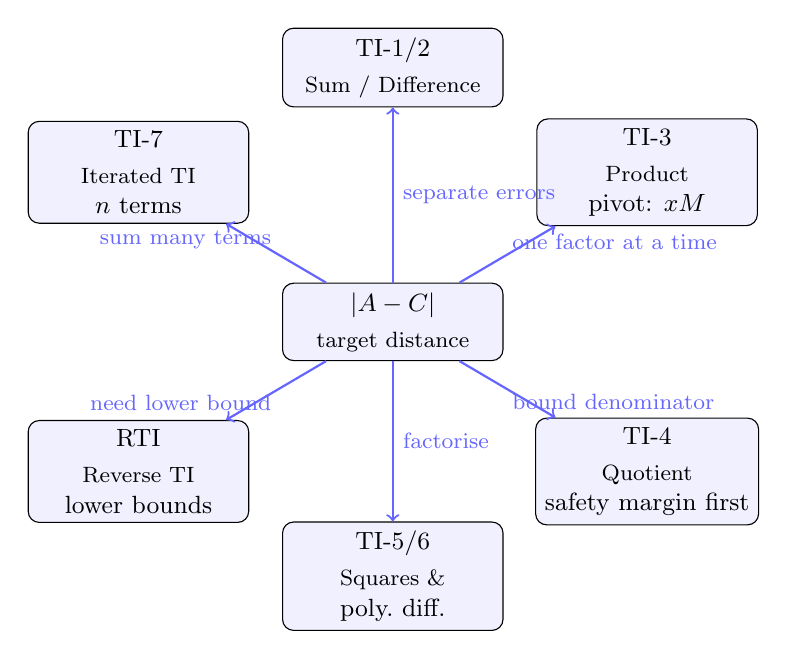
\begin{tikzpicture}[
  box/.style={rectangle,draw,rounded corners=4pt,fill=blue!6,
              minimum width=2.8cm,minimum height=0.85cm,
              align=center,font=\small},
  arr/.style={->,thick,blue!60},
  scale=0.95
]
  \node[box] (core) at (0,0)
    {$|A-C|$\\[2pt]\footnotesize target distance};

  \node[box] (sum)  at (0, 3.4)
    {TI-1/2\\[2pt]\footnotesize Sum / Difference};
  \node[box] (prod) at (3.4, 2.0)
    {TI-3\\[2pt]\footnotesize Product\\pivot: $xM$};
  \node[box] (quot) at (3.4,-2.0)
    {TI-4\\[2pt]\footnotesize Quotient\\safety margin first};
  \node[box] (sq)   at (0,-3.4)
    {TI-5/6\\[2pt]\footnotesize Squares \&\\poly.\ diff.};
  \node[box] (iter) at (-3.4,2.0)
    {TI-7\\[2pt]\footnotesize Iterated TI\\$n$ terms};
  \node[box] (rev)  at (-3.4,-2.0)
    {RTI\\[2pt]\footnotesize Reverse TI\\lower bounds};

  \draw[arr] (core) -- (sum)  node[midway,right]{\footnotesize separate errors};
  \draw[arr] (core) -- (prod) node[midway,above right=-2pt]
                               {\footnotesize one factor at a time};
  \draw[arr] (core) -- (quot) node[midway,below right=-2pt]
                               {\footnotesize bound denominator};
  \draw[arr] (core) -- (sq)   node[midway,right]{\footnotesize factorise};
  \draw[arr] (core) -- (iter) node[midway,above left=-2pt]
                               {\footnotesize sum many terms};
  \draw[arr] (core) -- (rev)  node[midway,below left=-2pt]
                               {\footnotesize need lower bound};
\end{tikzpicture}
\caption{The seven toolkit rules as different strategies for resolving
a single target distance. The choice of branch is determined by the
algebraic structure of the expression.}
\end{figure}

\begin{remark*}[How to use this diagram when reading a proof]
When you encounter a bounding inequality in any proof, locate the
target expression in the centre of this diagram and ask which branch
was taken. This turns an opaque inequality into a recognisable move
from a known toolkit.
After enough practice, you will see the branch before the inequality
is even written — the algebraic form of the expression announces
which tool will be applied.
\end{remark*}

\begin{remark*}[Bounds are designed to be generous]
A theme running through every section of this chapter is that analysis
bounds are deliberately \emph{over-generous}.
The product decomposition double-counts the corner square.
The sum bound ignores cancellation between errors of opposite sign.
The $|M| + 1$ trick in the denominator is larger than necessary.
The $\varepsilon/n$ split allocates equal budget to terms that may need
unequal amounts.

None of this is sloppiness.
It is a principled design choice: we trade tightness for linearity,
and linearity for mechanical closure.
A bound that is slightly too large is still a valid bound, and a valid
bound that closes by routine procedure is worth far more than a tight
bound that requires fresh reasoning every time.

The inequality sign is not a confession of imprecision.
It is the mechanism that makes analysis proofs reusable.
\end{remark*}